\documentclass[12pt]{article}
\usepackage[dvipsnames]{xcolor}
\usepackage{fullpage,enumitem,amsmath,amssymb,graphicx}
\usepackage[T1]{fontenc}
\usepackage{tikz} 
\usepackage{lipsum}
\usepackage{listings}
\usepackage{float}
\usepackage{scrextend}
\usepackage{multicol}
\usepackage{subcaption}
\usepackage[normalem]{ulem}
\setlength{\columnsep}{1cm}
\usepackage{hyperref}
\usepackage{fancyvrb}
\usepackage{xcolor}
\hypersetup{
    colorlinks=true,
    linkcolor=blue,
    filecolor=magenta,      
    urlcolor=cyan,
    pdftitle={Overleaf Example},
    pdfpagemode=FullScreen,
    }

\newenvironment{subs}
  {\adjustwidth{3em}{0pt}}
  {\endadjustwidth}

\title{\vspace{-1cm} \Huge Project 1 - Favor for the Ringmaster
\\ \LARGE CmpE 230,  Systems Programming, Spring 2024 }
\author{
  Instructor: Can Özturan\\
  TAs: Gökçe Uludoğan, Goshgar İsmayilov\\
  SA: Işıl Su Karakuzu
}
\date{Due: March 31, 2024, 23:59 (Strict)}

\begin{document}
  \maketitle
  \section{Introduction}

\indent \indent 
One morning, you wake up and find yourself in North Oxford in 1940, right next to J.R.R. Tolkien's house, serving as his assistant.
\\\\
\indent J.R.R. Tolkien is writing his novel, `The Lord of the Rings'. Since it's a bit lengthy and challenging to manage, he asks one of his favorite assistants —you— to help him keep track of the characters' inventories.
\\\\
\indent Your duty is to invent something for Tolkien that keeps track of characters' inventories. As a time traveler familiar with the wonders of the C programming language, you decide to write an interpreter using C for Tolkien.
\\

\begin{figure}[h]
        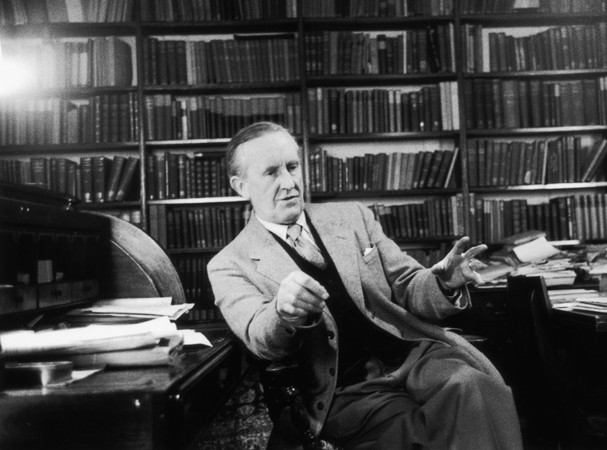
\includegraphics[width=1\linewidth, height=6cm, keepaspectratio]{tolkien.jpeg}
        \centering
        \captionsetup{justification=centering}
        \caption{Tolkien requests a favor from you.}
    \label{fig:image2}
\end{figure}


\pagebreak
\section{Details}
\indent Examining our C program, it remains ready to receive inputs until the user enters the "exit" command. This tool handles three input types:
\begin{itemize}
    \item \textbf{Sentence:} Providing details about characters and their inventories. When provided with a valid sentence, the program outputs "OK"; otherwise, it prints "INVALID". However, the program should continue to run.
    \item \textbf{Question:} Prompting the program to find information for J.R.R. Tolkien's writing. The program accurately provides answers to questions.
    \item \textbf{Exit Command:} The program terminates.
\end{itemize}


\subsection{Sentences}

\indent Our constructed language sentences are formed using these types:

\subsubsection{Entities}

\begin{itemize}
\item \textbf{Subject(s):} Describes entities or things of interest. Each subject is a single word that can contain uppercase and lowercase letters, including underscores. Multiple subjects can be detailed, separated by `and'. For example:

\begin{itemize}

    \item Gandalf
    \item Frodo Baggins (INVALID: Contains space)
    \item Frodo\_Baggins
    \item Aragorn and Sauron
    \item Sam and Pippin and Mary
    \item Gandalf1907 (INVALID: Contains digits) \\
\end{itemize}

 \item \textbf{Item(s):} Refers to objects associated with a non-negative integer quantity. Each item is a single word that can contain uppercase and lowercase letters, including underscores. Multiple items can be specified, \textbf{each accompanied by a non-negative integer}, and separated by `and'. The term \textbf{does not get a plural suffix `s'} when it is specified as plural. For example:
\begin{itemize}
    \item Narsil (INVALID: Missing quantity)
    \item 2 Narsil
    \item 1 Palantir and 0 elven\_rope and 44 Ormal
    \item 1 Palantir and elven\_rope and 44 Ormal (INVALID: Missing quantity )
    \\

\end{itemize}
\item \textbf{Location:} Represents a place or setting using a single word that can contain uppercase and lowercase letters, including underscores. \textbf{Describing multiple locations is not allowed.} For example:
\begin{itemize}

    \item Gondor
    \item Isendar and Rivendell (INVALID: Multiple locations)
    \item Minas\_Tirith

\end{itemize}

\end{itemize}

\noindent These entity names \textbf{must not contain any special keywords} defined in the language. \\ 

\noindent \underline{Keywords:} \{sell, buy, go, to, from, and, at, has, if, less, more, than, exit, where, total, who, NOBODY, NOTHING, NOWHERE\} \\

\noindent In test cases, each name will belong to only one type of entity. For example, in a given scenario, `Frodo' won't be assigned as both a subject name and an item name. \\

\noindent If the given entities do not follow these rules, the constructed sentence must be INVALID, and the program should print INVALID.

\subsubsection{Actions}

\begin{itemize}

\item \textbf{"buy":} Subject(s) acquire item(s) from an \textbf{infinite} source. After this action, the quantity of purchased item(s) in the inventory is increased. For example:\\\\
Subject(s) \textbf{buy} Item(s)
        \begin{itemize}
        \item Gandalf \textbf{buy} 5 bread
        \item Gandalf and Gollum \textbf{buy} 2 bread
        \item Gandalf and Gollum \textbf{buy} 6 bread and 4 water \\

        \end{itemize}
        
\item \textbf{"buy ... from":} Subject(s) acquire item(s) from another subject, which is a \textbf{finite} source. If there are multiple buyers, the seller provides the given amount of items to each buyer. The buy operation is done only if the seller has enough items for all buyers. Otherwise, do nothing. In the buy action, there cannot be more than one seller subject. The seller and buyer cannot be the same person. After this action, the quantity of purchased item(s) in the inventory for buyers is increased, while for the seller, it is decreased. For example:\\\\
Subject(s) \textbf{buy} Item(s) \textbf{from} Subject
        \begin{itemize}

        \item Gandalf \textbf{buy} 5 bread \textbf{from} Aragorn
        \item Gandalf and Gollum \textbf{buy} 2 bread \textbf{from} Gollum (INVALID: Subject serving as both the seller and the buyer)
        \item Gandalf and Gollum \textbf{buy} 6 bread and 4 water \textbf{from} Aragorn
        \item Gandalf and Gollum \textbf{buy} 6 bread \textbf{from} Aragorn and Legolas (INVALID: Multiple sellers) 

        \end{itemize}
\item \textbf{"sell":} Subject(s) give item(s) to an infinite source. After this action, the quantity of sold item(s) in the inventory is decreased. If the subject(s) do not have enough item(s), do nothing. For example: \\\\
Subject(s) \textbf{sell} Item(s)
\begin{itemize}

        \item Gandalf \textbf{sell} 5 bread
        \item Gandalf and Gollum \textbf{sell} 2 bread
        \item Gandalf and Gollum \textbf{sell} 6 bread and 4 water

\end{itemize}

\item \textbf{"sell ... to":} Subject(s) which are a \textbf{finite} source, provide item(s) to another subject. If there are multiple sellers, each provides the given amount of items to the buyer. The sell operation is done only if all the sellers have enough items for the buyer. Otherwise, do nothing. In the sell action, there cannot be more than one buyer subject. The seller and buyer cannot be the same person. After this action, the quantity of sold item(s) in the inventory for sellers is decreased, while for the buyer, it is increased. For example: \\\\
Subject(s) \textbf{sell} Item(s) \textbf{to} Subject
        \begin{itemize}

        \item Gandalf \textbf{sell} 5 bread \textbf{to} Aragorn
\item Gandalf and Gollum \textbf{sell} 2 bread \textbf{to} Gollum (INVALID: Subject serving as both the seller and the buyer)
\item Gandalf and Gollum \textbf{sell} 6 bread and 4 water \textbf{to} Aragorn
\item Gandalf and Gollum \textbf{sell} 6 bread \textbf{to} Aragorn and Legolas (INVALID: Multiple buyers)

        \end{itemize}
\item \textbf{"go to":} Subject(s) move to a location. It is possible for subject(s) to move to their current location. Subject(s) cannot go to multiple locations at the same time. Remember, describing multiple locations is not allowed. For example:\\\\
Subject(s) \textbf{go to} Location
        \begin{itemize}
        \item Gandalf \textbf{go to} Shire
        \item Frodo and Sam \textbf{go to} Mordor
        \item Frodo \textbf{go to} Mordor and Isengard (INVALID: Multiple locations) 
        \end{itemize}
\end{itemize}

\noindent It is possible to create action series called Action(s). It starts with a \textbf{single action}, followed by an `and' and additional actions, optionally. Each action in an action series is performed from left to right separately.\\

\noindent \textbf{Action(s):} Frodo and Sam go to Mordor \textbf{and} Gandalf sell 5 bread and 3 sword to Aragorn \textbf{and} Legolas buy 3 hairclip\\

\noindent At the beginning, each subject has \textbf{0 items} in their inventory and is located in \textbf{NOWHERE}. 

\subsubsection{Conditions}
\begin{itemize}
    \item {\textbf{"at":} Specifies the location where the subject(s) are present. For this condition to be true, all subjects mentioned should be at the specified location. Remember, describing multiple locations is not allowed. For example:\\\\
    Subject(s) \textbf{at} Location
    \begin{itemize}
        \item Gandalf \textbf{at} Shire
        \item Frodo and Sam \textbf{at} Mordor
        \item Frodo \textbf{at} Mordor and Isengard (INVALID: Multiple locations) 
    \end{itemize}
    
    }

\item {\textbf{"has":} Indicates possession, stating that the subject has a \textbf{certain} quantity of an item. For this condition to be true, each subject mentioned should have the specified amount of the items exactly. For example: \\\\
Subject(s) \textbf{has} Item(s)
\begin{itemize}
        \item Gandalf \textbf{has} 5 bread
        \item Gandalf and Gollum \textbf{has} 2 bread
\item Gandalf and Gollum \textbf{has} 6 bread and 4 water
\item Gandalf \textbf{has} bread (INVALID: Missing quantity)

    \end{itemize}
}

\item {\textbf{"has less than":} Describes a condition where the subject possesses an amount of an item that is less than a specified value. For this condition to be true, each subject mentioned should have less than the specified amount of the items. For example: \\\\
Subject(s) \textbf{has less than} Item(s)
\begin{itemize}
        \item Gandalf \textbf{has less than} 10 ring
        \item Gandalf and Gollum \textbf{has less than} 5 sword and 3 map
        \item Gandalf \textbf{has less than} \space \space    (INVALID: Missing items)

    \end{itemize}
}

\item {\textbf{"has more than":} Describes a condition where the subject possesses an amount of an item that is greater than a specified value. For this condition to be true, each subject mentioned should have more than the specified amount of the items. For example: \\\\
Subject(s) \textbf{has more than} Item(s)
\begin{itemize}
        \item Gandalf \textbf{has more than} 10 ring
        \item Gandalf and Gollum \textbf{has more than} 5 sword and 3 map
        \item Gandalf \textbf{has more than} ring (INVALID: Missing quantity)

    \end{itemize}
}
\end{itemize}

\noindent These condition types are exclusively used within if statements and \textbf{cannot exist independently}.\\

\noindent It is possible to create condition series called Condition(s). It starts with a \textbf{single condition}, followed by an `and' and additional conditions, optionally. Each condition in a condition series is assessed from left to right separately. If all conditions are true, the overall condition is considered true. If any of the conditions is false, the overall condition is considered false.\\

\noindent \textbf{Condition(s):} Frodo at Mordor \textbf{and} Gandalf has lower than 10 ring \textbf{and} Aragorn and Legolas has 5 map

\subsubsection{Constructing a Sentence}
Sentences can be made in 3 different ways:

\begin{itemize}
    \item \textbf{Basic Sentences:} Composed of a set of actions that the program will perform. For example : \\\\
    Actions(s)
    \begin{itemize}
        \item Legolas and Gimli go to Rivendell \textbf{and} Legolas and Gimli buy 2 elixir and 1 map from Arwen
\item Aragorn and Frodo sell 3 dagger to Gimli \textbf{and} Pippin go to Shire
\item Saruman sell 4 staff to Frodo
\item Aragorn and Legolas go to Lothlorien \textbf{and} Aragorn and Legolas buy 2 lembas\_bread and 1 bow from Galadriel \textbf{and} Gimli sell 3 axe
    \end{itemize}
    \item \textbf{Conditional Sentences:} Include actions that will only be executed if specific conditions are met. If all given conditions are true, then all actions will occur from left to right. For example: \\\\
    Action(s) \textbf{if} Condition(s) 
    \begin{itemize}
        \item Gandalf sell 3 sword to Aragorn \textbf{if} Frodo has more than 5 ring and Legolas and Gimli at Rivendell
        \item Frodo and Sam go to Mount\_Doom \textbf{if} Gollum has 1 the\_One\_Ring and Gandalf has less than 3 staff and 2 bread
        \item Frodo and Sam go to Mordor and Gandalf sell 5 bread \textbf{if} Frodo has more than 3 ring

    \end{itemize}
    \item \textbf{Sequential Sentences:} Combine actions and conditions in a sequence, allowing for a series of linked instructions. Each sentence is executed separately, following a left-to-right order. For example: \\\\
    Sentence-1 \textbf{and} Sentence-2 \textbf{and} Sentence-3
    \begin{itemize}
        \item \color{blue} Frodo and Sam go to Bree and Frodo buy 3 map from Aragorn and Sam sell 2 dagger to Legolas if Frodo has more than 2 ring and Legolas and Gimli at Bree \color{black} \textbf{and} \color{ForestGreen} Frodo and Sam go to Rivendell if Aragorn has 5 map and Frodo has less than 5 potion and Sam has 3 dagger \color{black} \textbf{and} \color{RedViolet} Frodo sell 1 potion to Arwen and Legolas and Gimli go to Rivendell
    \end{itemize}
\end{itemize}

\subsection{Questions}
\begin{itemize}
    \item \textbf{Quantity asking (total ... ?):} It inquires about the total count of a specific item for the mentioned subjects. The question is restricted to a single item and cannot involve multiple items. The result integer should be returned in a single line as the answer. For example: \\\\
    Subject(s) \textbf{total} Item \textbf{?} \\\\ \textit{Example:} Gandalf and Frodo \textbf{total} ring \textbf{?} $\rightarrow$ 5 
    
\item \textbf{Location asking (where ?):} 
It inquires about the current location of a specified subject. The question will involve only one subject. For example: \\\\
Subject \textbf{where} \textbf{?} \\\\
\textit{Example:} Frodo \textbf{where} \textbf{?} $\rightarrow$ Rivendell 

\item \textbf{Presence in a location (Who at ... ?):} It seeks information about the subjects present in a specified location. Remember, describing multiple locations is not allowed. The response should provide a list of all subjects located in the given place in a single line, separated by `and'. The order of the answer does not matter; any order will be accepted. If there is no one at the specified location, the output should be "NOBODY". For example: \\\\
\textbf{Who at} Location \textbf{?} \\\\
\textit{Example:} \textbf{Who at} Rivendell \textbf{?} $\rightarrow$ Frodo and Gimli 

\item  \textbf{Inventory inquiry (total ?):} This question type aims to retrieve information about the complete inventory of the specified subject. The question is not limited to a specific item but encompasses all items present in the subject's inventory. The result should provide details about each item, including its name and quantity, in a single line as the answer, separated by `and'. There will be only one subject asked at each of this question type. The order of the answer does not matter; any order will be accepted. Printing items with a quantity of 0 in the inventory will not be accepted. If a subject doesn't have any items in their inventory, the output should be "NOTHING". For example: \\\\
Subject \textbf{total ?} \\\\
\textit{Example:} Gandalf \textbf{total ?} $\rightarrow$ 5 ring and 3 staff and 2 bread

\end{itemize}

\subsection{Exit Command}

When the "exit" command is entered, the program should terminate without encountering any errors.

\section{Input \& Output}
\begin{itemize}
\item There will be no expressions or assignments with a result that exceeds a 32-bit number. 
\item All words are \textbf{case-sensitive}; For example: `Shire' and `shire' are not the same.
\item Sentences or questions will consist of 1024 characters at most.
\item Each input should be read after printing "$>>$ " to the terminal.
\item There might be multiple spaces between words; it's valid for both input and output. There won't be a test case with escape sequences like \textbackslash{r} and \textbackslash{t}. Only white-space and \textbackslash{n} at the end of the line will be given in the input.
\item If a sentence or question is INVALID, no actions should be executed based on the given input, even if it contains correct sentences.
\item The execution of the program will be done through the interpreter screen working in the terminal - in other words, it won't be a file-based program. It should work just like the Python interpreter. 
\item Remember, when provided with a valid sentence, the program outputs "OK"; otherwise, it prints "INVALID". However, the program should continue to run.
\item An empty line will not be given as input.
\item Test cases will not exceed a maximum of \textbf{128 lines}. Focus on \textbf{code correctness rather than optimization} for this project.

\end{itemize}
\subsection{Examples to Rule Them All}

\indent These examples address the mentioned details but do not cover all edge cases.

\begin{itemize}
    \item \textbf{Example 1} : General expectations from the program.{
\begin{verbatim}
$ make
$ ./ringmaster
>> Frodo go to Rivendell
OK
>> who at Shire ?
NOBODY
>> Frodo    where ?
Rivendell
>> Frodo sell 2 bread to Sam
OK 
>> Sam total ?
NOTHING (Explanation: Frodo does not have enough bread to sell to Sam.)
>> Frodo and Sam buy 3 bread and 2 ring
OK
>> Sam sell 1 ring to Sauron
OK
>> Sauron where ?
NOWHERE
>> Sam total ?
3 bread and 1 ring
>> Frodo buy 2 palantir and Frodo go to NOWHERE
INVALID (Explanation: Frodo can not go to a place which is a keyword.)
>> Frodo total palantir ?
0
>> Frodo total Bread ?
0
>> Frodo go to mount_doom and Gandalf buy 3 arrow if Sauron has 1 ring and Frodo
at Rivendell
OK
>> who at mount_doom ?
Frodo
>> Legolas buy 100 hairclip from Arwen if Galadriel at NOWHERE
INVALID (Explanation: Even though Galadriel is at NOWHERE, her initial location,
NOWHERE is a keyword and therefore cannot be specified in sentences or questions
as entities. But keywords such as NOWHERE, NOTHING, NOBODY can be at the 
program's output.)
>> Legolas total hairclip ?
0
>> Legolas buy 100 hairclip from Arwen if Gandalf has more than 2 arrow
OK
>> Legolas total hairclip ?
0 (Explanation: Even though the previous sentence is correct, Arwen doesn't have
enough hairclips to give to Legolas.)
>> exit
\end{verbatim}
}

\item \textbf{Example 2} : Basic transaction process with one or more items.{
\begin{verbatim}
$ make
$ ./ringmaster
>> Galadriel and Elrond and Cirdan buy 100 Nenya and 100 Narya and 100 Vilya
OK
>> Balrog and Saruman buy 10 Vilya and 10 Narya from Cirdan
OK
>> Cirdan total ?
100 Nenya and 80 Vilya and 80 Narya
>> Balrog total ?
10 Narya and 10 Vilya
>> Balrog and Cirdan sell 10 Nenya to Legolas
OK
>> Legolas total Nenya ?
0 (Explanation: The previous statement is correct, but since Cirdan
doesn't have any Nenya rings, the action is canceled for both.)
>> Balrog and Cirdan sell 10 Vilya to Legolas
OK
>> Legolas total Vilya ?
20
>> Balrog and Cirdan total Narya ?
90
>> exit




\end{verbatim}}

\item \textbf{Example 3} : Entity names, question words and keywords are case-sensitive.{
\begin{verbatim}
>> someone go to somewhere and somebody buy 1 somethings and 2 SoMeTHiNG 
if someone has less than 2 somethings and 1 nothinG and 
someone go to home_of_someone if someone has 10 something
OK
>> someone where ?
somewhere
>> somebody where ?
NOWHERE
>> who at home_of_someone ?
NOBODY
>> everyone and somebody and someone go to everywhere and this is invalid 
if everyone at everywhere
INVALID
>> everyone where ?
NOWHERE
>> exit
\end{verbatim}}

\item \textbf{Example 4} : When there are not enough items, even if the other items are sufficient, the action is not carried out.{
\begin{verbatim}
>> Galadriel and Elrond buy 3 bread and 2 map
OK
>> Galadriel sell 3 bread and 3 map
OK
>> Galadriel total ?
3 bread and 2 map
>> Galadriel sell 3 bread and 3 map to Cirdan
OK
>> Galadriel total ?
3 bread and 2 map
>> Cirdan total ?
NOTHING
>> exit





\end{verbatim}}
\end{itemize}

\section{Submission}

Your project will be tested automatically on \href{https://hub.docker.com/repository/docker/gokceuludogan/cmpe230_spring24}{the provided docker image}. Thus, it's important that you carefully follow the submission instructions. Instructions for setting up the development environment can be found at \href{https://github.com/bouncmpe230/docker-starter-course/}{this page}. The root folder for the project should be named according to your student id numbers. If you submit individually, name your root folder with your student id. If you submit as a group of two, name your root folder with both student ids separated by an underscore. You will compress this root folder and submit it with the \texttt{.zip} file format. Other archive formats will not be accepted. The final submission file should be in the form of either \texttt{2020400144.zip} or \texttt{2020400144\_2020400099.zip}. 
\\\\
\noindent You must create a Makefile in your root folder which creates a \texttt{ringmaster} executable in the root folder, do not include this executable in your submission, it will be generated with the \texttt{make} command using the Makefile. The \texttt{make} command should not run the executable, it should only compile your program and create the executable. 
\\\\
\noindent Additionally, submit your project to the Github Classroom assignment for this project to verify its structure and basic functionality. The link to join this assignment will be provided shortly.

\subsection*{Late Submission}
If the project is submitted late, the following penalties will be applied:
\begin{table}[H]
\centering
\begin{tabular}{|l|l|}
\hline
\textbf{Hours late}                       & \textbf{Penalty} \\ \hline
0  \textless \vspace{1pt} hours late  \textless{}=  24  & 25\%             \\ % congrats
24 \textless  \vspace{1pt} hours late  \textless{}=  48 & 50\%             \\
 hours late   \textgreater  \vspace{1pt}  48   & 100\%           \\ \hline

\end{tabular}
\end{table}



\section{Grading}
Your project will be graded according to the following criteria: 
\begin{itemize}
    \item \textbf{Code Comments (8\%): } Write code comments for discrete code behavior and method comments. This sub-grading evaluates the quality and quantity of comments included in the code. Comments are essential for understanding the code's purpose, structure, logic, and any complex algorithms or data structures used. The code should be easily readable and maintainable for future developers.\\\\\\
    \item \textbf{Documentation (12\%): } A written document describing how you implemented your project. This sub-grading assesses the quality and completeness of the written documentation accompanying the project. Good documentation should describe the purpose, design, and implementation details, as well as any challenges encountered and how they were addressed. The documentation should also include examples of input/output and how to use the program. Students should aim to write clear, concise, and well-organized documentation that effectively communicates the project's functionality and design decisions.
    \item \textbf{Implementation and Tests (80\%): } The submitted project should be implemented following the guidelines in this description and should pass testing. This sub-grading assesses the quality and correctness of the implementation.\\\\
    Grading the test cases will be straightforward: your score from the test cases will be determined by the formula:
    \center Total Correct Answers to Lines $/$ Total Lines Given
\end{itemize}
\section{Warnings}
\begin{itemize}

\item You can submit this project either individually or as a group of two. 

\item All source codes are checked automatically for similarity with other submissions and exercises from previous years. Make sure you write and submit your own code. Any sign of cheating will be penalized with an F grade.  

\item Do not use content from external AI tools directly in your code and documentation. Doing so will be viewed as plagiarism and thoroughly investigated.

\item Project documentation should be structured in a proper manner. The documentation must be submitted as a .pdf file, as well as in raw text format.

\item Make sure you document your code with necessary inline comments and use meaningful variable names. Do not over-comment, or make your variable names unnecessarily long. This is very important for partial grading. 

\item Do not start coding right away. Think about the structure of your program and the possible complications resulting from it before coding.

\item Questions about the project should be sent through the discussion forum on Piazza. 

\item There will be a time limit of 30 seconds for your program execution. Program execution consists of the total amount of time for all queries. This is not a strict time limit and the execution times may vary for each run. Thus, objections regarding time limits will be considered if necessary. 

\end{itemize}
\end{document}